\section{The training tool}
Here the appropriate way of using the training tool is explained in detail.

\subsection{Access}
The tool is a dynamic web page and can thus be accessed via browser.

\subsection{Uploading a CSV file in the tool}
The user will need to feed the tool a CSV file containing properly marked values for the algorithm the user has intention of training.

This can be done by selecting the "Select file" button, which will open a window from which the user will be able to select the CSV file he has intention of uploading.

\begin{figure}[H]
\centering
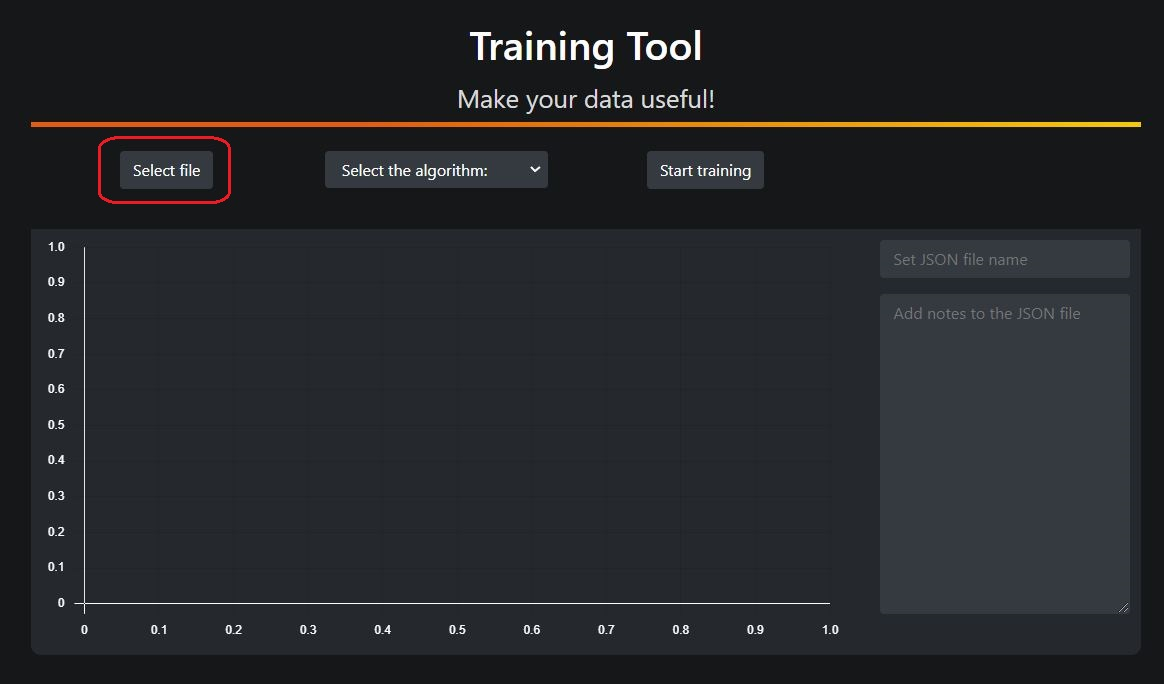
\includegraphics[scale=0.65]{img/tool/screen_1_tool.JPG}
\caption{CSV-File selector}
\end{figure}
\newpage

\subsection{Selection of the algorithm}
The user will have to choose between training a Support Vector Machine or a Linear Regression algorithm with the CSV file he has given to the tool.

To do this, the user can open a drop-down menu called "Select the algorithm" which displays the two algorithms that can be chosen. The preferred algorithm can at this point be selected.
\begin{figure}[H]
\centering
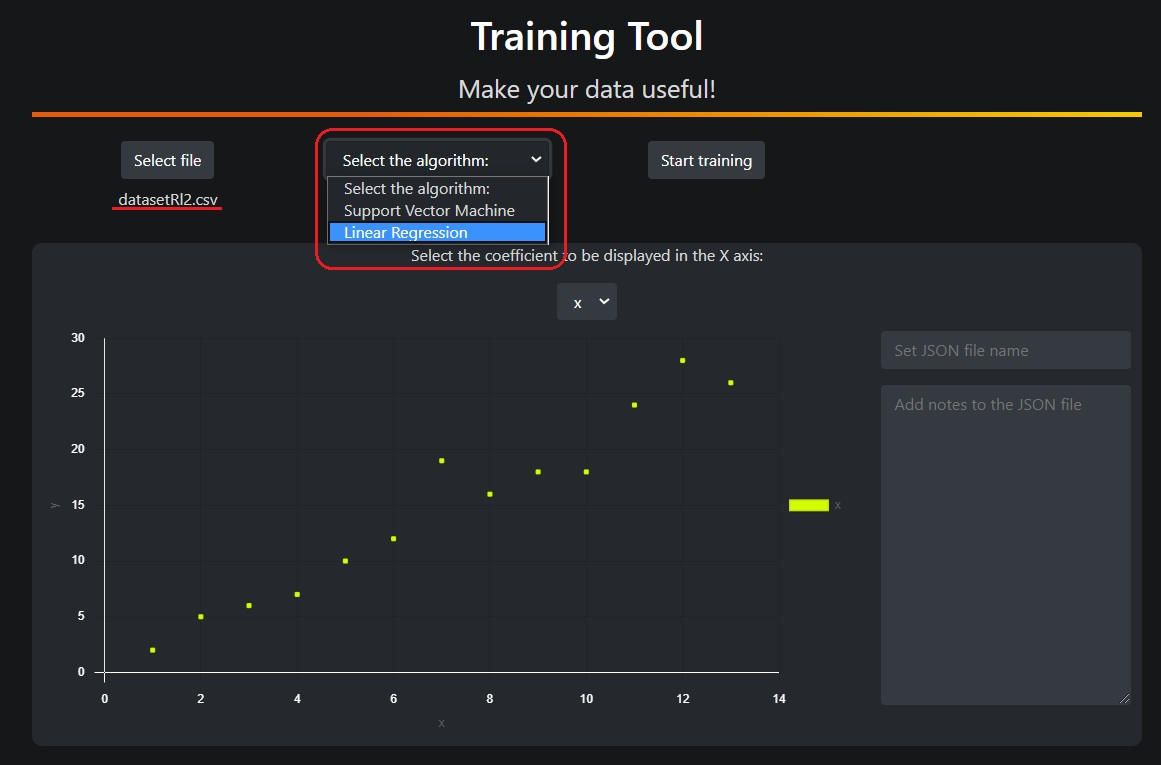
\includegraphics[scale=0.65]{img/tool/screen_2_tool.JPG}
\caption{Training algorithm selector}
\end{figure}
Should the user have uploaded training data incompatible with the selected algorithm, an error message will be displayed on selection of the "Start training" button.\newline
\begin{figure}[H]
\centering

\includegraphics[scale=0.65]{img/tool/error_alg.JPG}
\caption{Incompatible algorithm uploaded}
\end{figure}
\newpage
\subsection{Training operation}
The tool will now be able to perform the training operation by simply  having the user select the “Start training” button. The tool will now have produced a JSON file containing the values needed for use in the plug-in.
\begin{figure}[H]
\centering
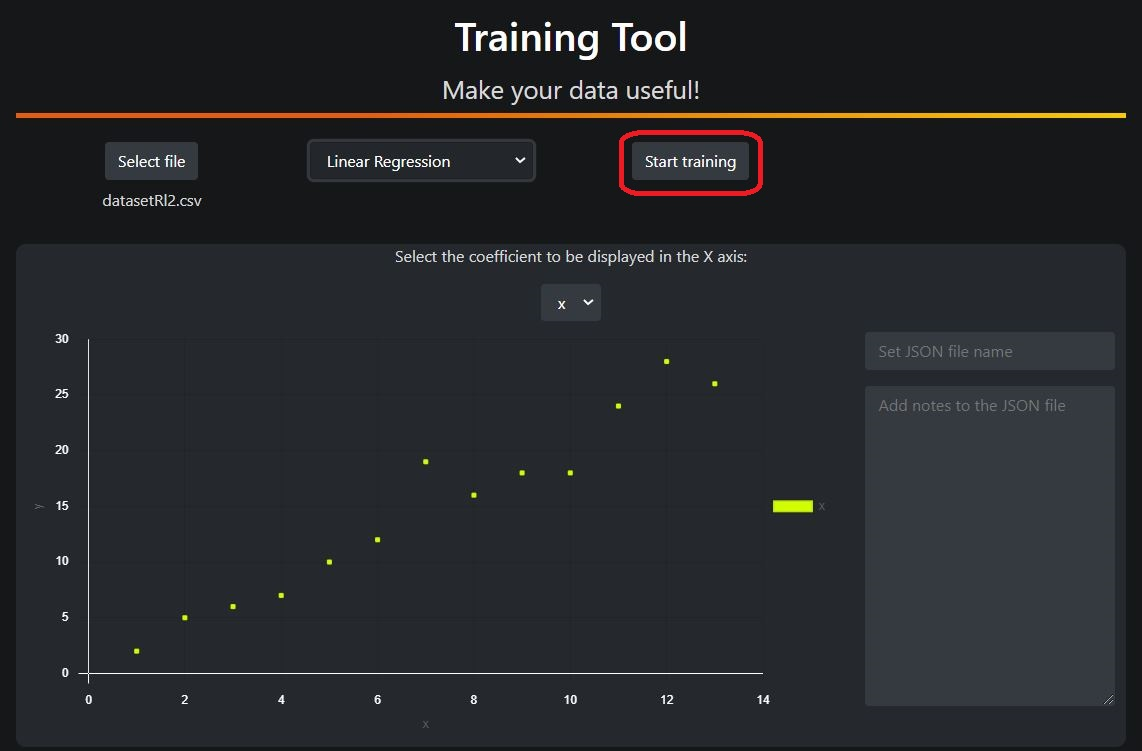
\includegraphics[scale=0.65]{img/tool/screen_3_1_tool.JPG}
\caption{Training operation with graphic point}
\end{figure}

A message will be displayed on selection of the "Start training" button if the training operation is successfully completed.
\newline
\begin{figure}[H]
\centering

\includegraphics[scale=0.65]{img/tool/screen_4_1_tool.JPG}
\caption{Training operation is successfully completed}
\end{figure}  
\newpage
\subsection{Obtaining the JSON file}
The user can now select the “Download” button, which will only appear once the training operation has ended successfully, and receive the JSON file.
\begin{figure}[H]
\centering
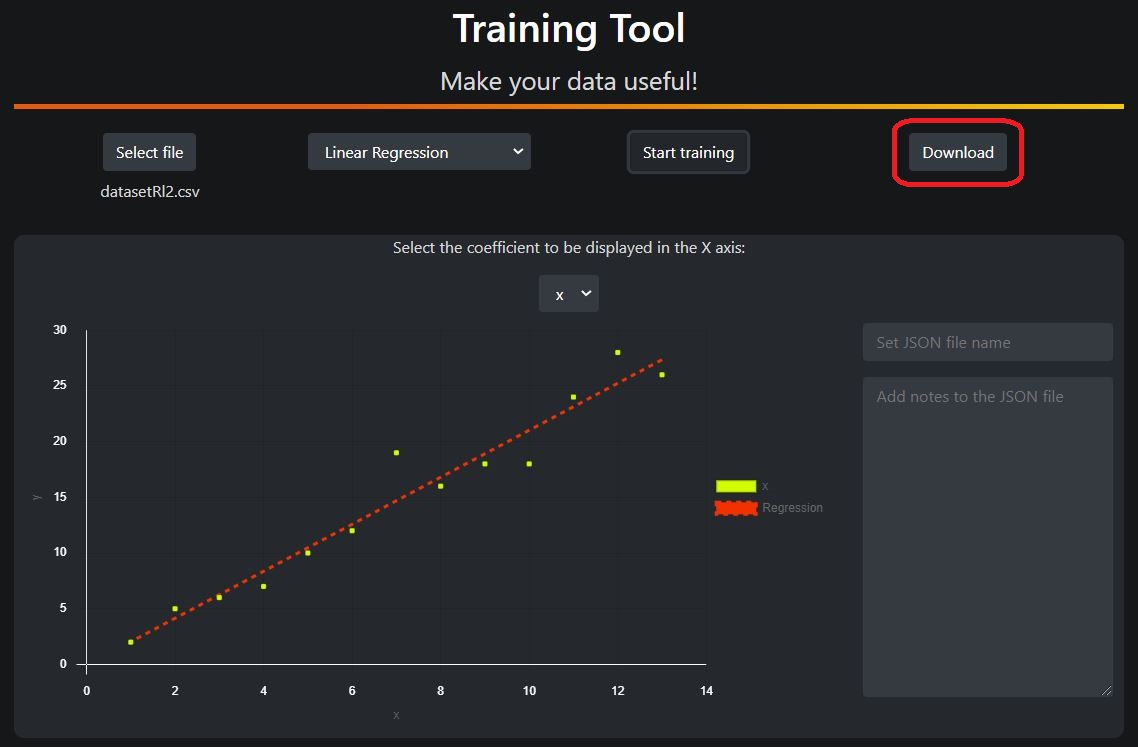
\includegraphics[scale=0.65]{img/tool/tool_5_1_tool.JPG}
\caption{The "Download" button is then clickable}
\end{figure} 
\newpage
\subsection{Info point}
Additional information can be accessed by selecting the "information" button, once selected a step-by-step guide will appear.

\begin{figure}[H]
\centering

\includegraphics[scale=0.65]{img/tool/screen_info_tool_2.JPG}
\caption{Info point button}
\end{figure} 

\subsubsection{Bug reporting}
The email address to which bug reports should be sent is displayed below the step-by-step guide, we will later explain in greater detail how to report a bug.

